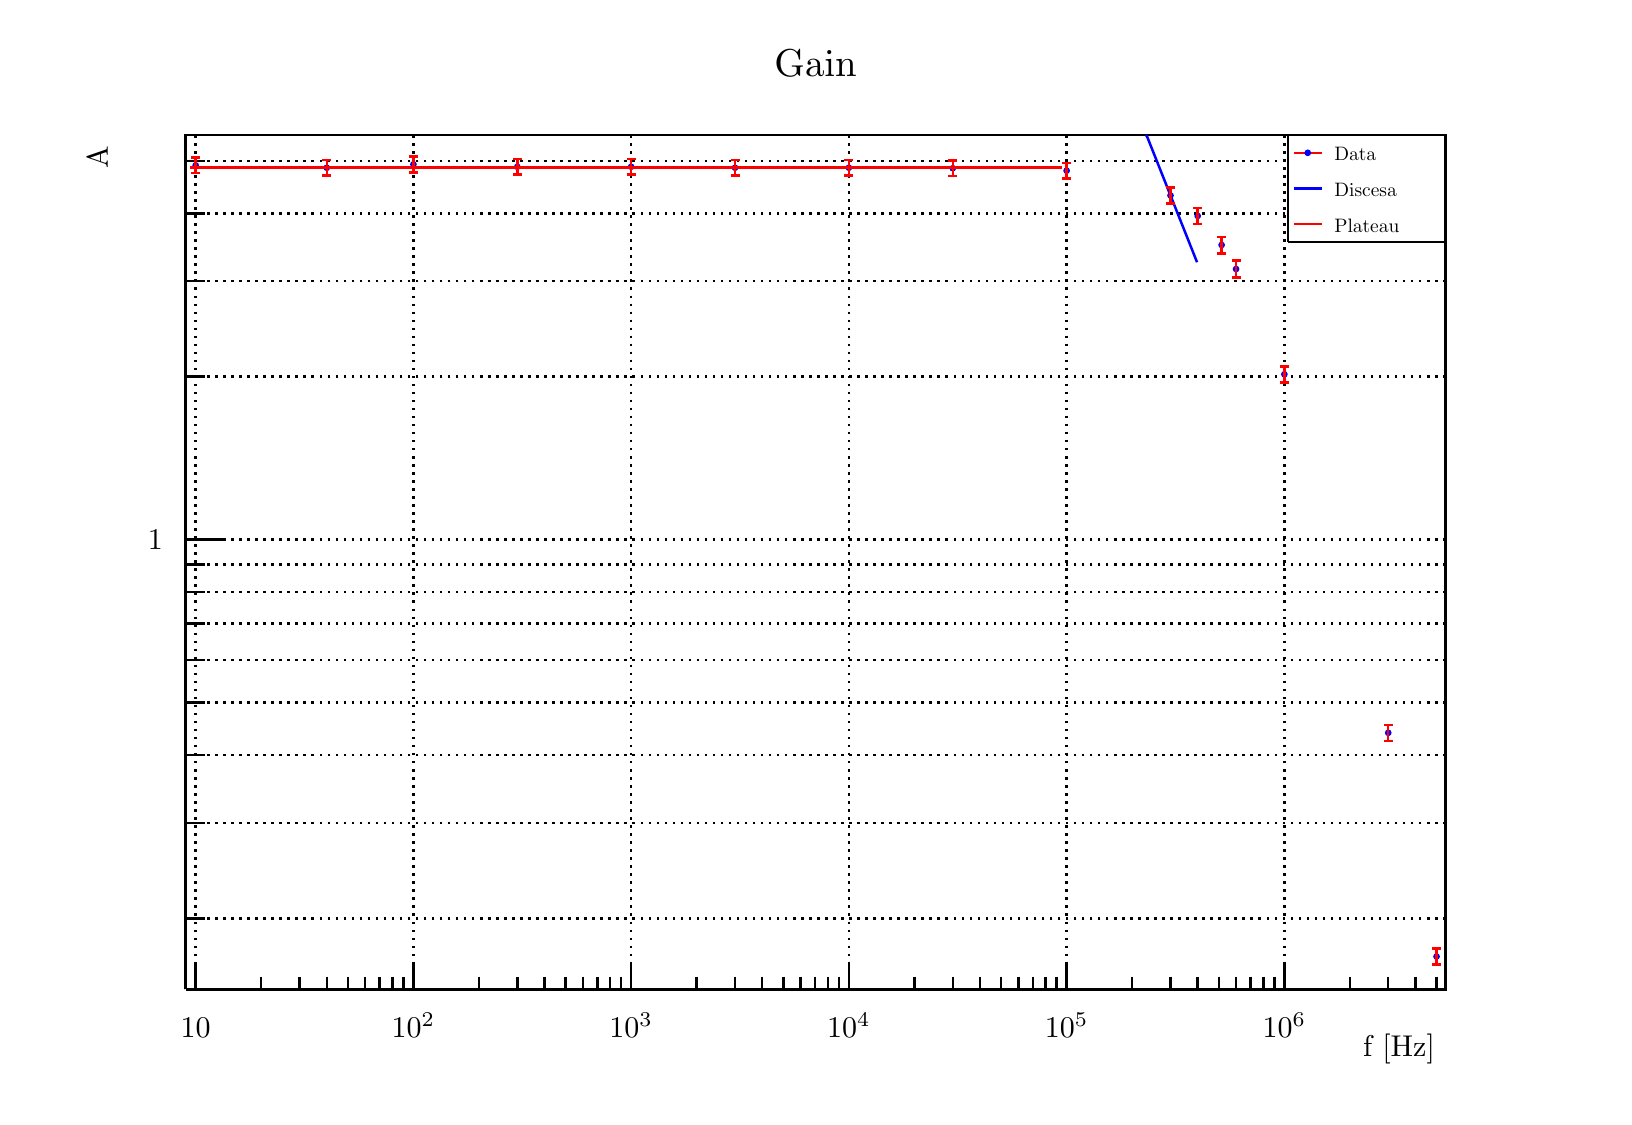
\begin{tikzpicture}
\pgfdeclareplotmark{cross} {
\pgfpathmoveto{\pgfpoint{-0.3\pgfplotmarksize}{\pgfplotmarksize}}
\pgfpathlineto{\pgfpoint{+0.3\pgfplotmarksize}{\pgfplotmarksize}}
\pgfpathlineto{\pgfpoint{+0.3\pgfplotmarksize}{0.3\pgfplotmarksize}}
\pgfpathlineto{\pgfpoint{+1\pgfplotmarksize}{0.3\pgfplotmarksize}}
\pgfpathlineto{\pgfpoint{+1\pgfplotmarksize}{-0.3\pgfplotmarksize}}
\pgfpathlineto{\pgfpoint{+0.3\pgfplotmarksize}{-0.3\pgfplotmarksize}}
\pgfpathlineto{\pgfpoint{+0.3\pgfplotmarksize}{-1.\pgfplotmarksize}}
\pgfpathlineto{\pgfpoint{-0.3\pgfplotmarksize}{-1.\pgfplotmarksize}}
\pgfpathlineto{\pgfpoint{-0.3\pgfplotmarksize}{-0.3\pgfplotmarksize}}
\pgfpathlineto{\pgfpoint{-1.\pgfplotmarksize}{-0.3\pgfplotmarksize}}
\pgfpathlineto{\pgfpoint{-1.\pgfplotmarksize}{0.3\pgfplotmarksize}}
\pgfpathlineto{\pgfpoint{-0.3\pgfplotmarksize}{0.3\pgfplotmarksize}}
\pgfpathclose
\pgfusepathqstroke
}
\pgfdeclareplotmark{cross*} {
\pgfpathmoveto{\pgfpoint{-0.3\pgfplotmarksize}{\pgfplotmarksize}}
\pgfpathlineto{\pgfpoint{+0.3\pgfplotmarksize}{\pgfplotmarksize}}
\pgfpathlineto{\pgfpoint{+0.3\pgfplotmarksize}{0.3\pgfplotmarksize}}
\pgfpathlineto{\pgfpoint{+1\pgfplotmarksize}{0.3\pgfplotmarksize}}
\pgfpathlineto{\pgfpoint{+1\pgfplotmarksize}{-0.3\pgfplotmarksize}}
\pgfpathlineto{\pgfpoint{+0.3\pgfplotmarksize}{-0.3\pgfplotmarksize}}
\pgfpathlineto{\pgfpoint{+0.3\pgfplotmarksize}{-1.\pgfplotmarksize}}
\pgfpathlineto{\pgfpoint{-0.3\pgfplotmarksize}{-1.\pgfplotmarksize}}
\pgfpathlineto{\pgfpoint{-0.3\pgfplotmarksize}{-0.3\pgfplotmarksize}}
\pgfpathlineto{\pgfpoint{-1.\pgfplotmarksize}{-0.3\pgfplotmarksize}}
\pgfpathlineto{\pgfpoint{-1.\pgfplotmarksize}{0.3\pgfplotmarksize}}
\pgfpathlineto{\pgfpoint{-0.3\pgfplotmarksize}{0.3\pgfplotmarksize}}
\pgfpathclose
\pgfusepathqfillstroke
}
\pgfdeclareplotmark{newstar} {
\pgfpathmoveto{\pgfqpoint{0pt}{\pgfplotmarksize}}
\pgfpathlineto{\pgfqpointpolar{44}{0.5\pgfplotmarksize}}
\pgfpathlineto{\pgfqpointpolar{18}{\pgfplotmarksize}}
\pgfpathlineto{\pgfqpointpolar{-20}{0.5\pgfplotmarksize}}
\pgfpathlineto{\pgfqpointpolar{-54}{\pgfplotmarksize}}
\pgfpathlineto{\pgfqpointpolar{-90}{0.5\pgfplotmarksize}}
\pgfpathlineto{\pgfqpointpolar{234}{\pgfplotmarksize}}
\pgfpathlineto{\pgfqpointpolar{198}{0.5\pgfplotmarksize}}
\pgfpathlineto{\pgfqpointpolar{162}{\pgfplotmarksize}}
\pgfpathlineto{\pgfqpointpolar{134}{0.5\pgfplotmarksize}}
\pgfpathclose
\pgfusepathqstroke
}
\pgfdeclareplotmark{newstar*} {
\pgfpathmoveto{\pgfqpoint{0pt}{\pgfplotmarksize}}
\pgfpathlineto{\pgfqpointpolar{44}{0.5\pgfplotmarksize}}
\pgfpathlineto{\pgfqpointpolar{18}{\pgfplotmarksize}}
\pgfpathlineto{\pgfqpointpolar{-20}{0.5\pgfplotmarksize}}
\pgfpathlineto{\pgfqpointpolar{-54}{\pgfplotmarksize}}
\pgfpathlineto{\pgfqpointpolar{-90}{0.5\pgfplotmarksize}}
\pgfpathlineto{\pgfqpointpolar{234}{\pgfplotmarksize}}
\pgfpathlineto{\pgfqpointpolar{198}{0.5\pgfplotmarksize}}
\pgfpathlineto{\pgfqpointpolar{162}{\pgfplotmarksize}}
\pgfpathlineto{\pgfqpointpolar{134}{0.5\pgfplotmarksize}}
\pgfpathclose
\pgfusepathqfillstroke
}
\definecolor{c}{rgb}{1,1,1};
\draw [color=c, fill=c] (0,0) rectangle (20,13.5632);
\draw [color=c, fill=c] (2,1.35632) rectangle (18,12.2069);
\definecolor{c}{rgb}{0,0,0};
\draw [c,line width=0.9] (2,1.35632) -- (2,12.2069) -- (18,12.2069) -- (18,1.35632) -- (2,1.35632);
\definecolor{c}{rgb}{1,1,1};
\draw [color=c, fill=c] (2,1.35632) rectangle (18,12.2069);
\definecolor{c}{rgb}{0,0,0};
\draw [c,line width=0.9] (2,1.35632) -- (2,12.2069) -- (18,12.2069) -- (18,1.35632) -- (2,1.35632);
\draw [c,line width=0.9] (2,1.35632) -- (18,1.35632);
\draw [c,dotted,line width=0.9] (2.12653,12.2069) -- (2.12653,1.35632);
\draw [c,dotted,line width=0.9] (4.89177,12.2069) -- (4.89177,1.35632);
\draw [c,dotted,line width=0.9] (7.657,12.2069) -- (7.657,1.35632);
\draw [c,dotted,line width=0.9] (10.4222,12.2069) -- (10.4222,1.35632);
\draw [c,dotted,line width=0.9] (13.1875,12.2069) -- (13.1875,1.35632);
\draw [c,dotted,line width=0.9] (15.9527,12.2069) -- (15.9527,1.35632);
\draw [c,line width=0.9] (2,1.35632) -- (2,12.2069);
\draw [c,dotted,line width=0.9] (18,2.25939) -- (2,2.25939);
\draw [c,dotted,line width=0.9] (18,3.47074) -- (2,3.47074);
\draw [c,dotted,line width=0.9] (18,4.3302) -- (2,4.3302);
\draw [c,dotted,line width=0.9] (18,4.99685) -- (2,4.99685);
\draw [c,dotted,line width=0.9] (18,5.54154) -- (2,5.54154);
\draw [c,dotted,line width=0.9] (18,6.00207) -- (2,6.00207);
\draw [c,dotted,line width=0.9] (18,6.401) -- (2,6.401);
\draw [c,dotted,line width=0.9] (18,6.75288) -- (2,6.75288);
\draw [c,dotted,line width=0.9] (18,7.06765) -- (2,7.06765);
\draw [c,dotted,line width=0.9] (18,9.13846) -- (2,9.13846);
\draw [c,dotted,line width=0.9] (18,10.3498) -- (2,10.3498);
\draw [c,dotted,line width=0.9] (18,11.2093) -- (2,11.2093);
\draw [c,dotted,line width=0.9] (18,11.8759) -- (2,11.8759);
\draw [c,line width=0.9] (2,1.35632) -- (18,1.35632);
\draw [anchor= east] (18,0.596782) node[scale=1.08496, color=c, rotate=0]{f [Hz]};
\draw [c,line width=0.9] (2.12653,1.68184) -- (2.12653,1.35632);
\draw [anchor=base] (2.12653,0.742586) node[scale=1.08496, color=c, rotate=0]{10};
\draw [c,line width=0.9] (2.95895,1.51908) -- (2.95895,1.35632);
\draw [c,line width=0.9] (3.44588,1.51908) -- (3.44588,1.35632);
\draw [c,line width=0.9] (3.79137,1.51908) -- (3.79137,1.35632);
\draw [c,line width=0.9] (4.05935,1.51908) -- (4.05935,1.35632);
\draw [c,line width=0.9] (4.2783,1.51908) -- (4.2783,1.35632);
\draw [c,line width=0.9] (4.46343,1.51908) -- (4.46343,1.35632);
\draw [c,line width=0.9] (4.62379,1.51908) -- (4.62379,1.35632);
\draw [c,line width=0.9] (4.76524,1.51908) -- (4.76524,1.35632);
\draw [c,line width=0.9] (4.89177,1.68184) -- (4.89177,1.35632);
\draw [anchor=base] (4.89177,0.742586) node[scale=1.08496, color=c, rotate=0]{$10^{2}$};
\draw [c,line width=0.9] (5.72419,1.51908) -- (5.72419,1.35632);
\draw [c,line width=0.9] (6.21112,1.51908) -- (6.21112,1.35632);
\draw [c,line width=0.9] (6.55661,1.51908) -- (6.55661,1.35632);
\draw [c,line width=0.9] (6.82458,1.51908) -- (6.82458,1.35632);
\draw [c,line width=0.9] (7.04354,1.51908) -- (7.04354,1.35632);
\draw [c,line width=0.9] (7.22866,1.51908) -- (7.22866,1.35632);
\draw [c,line width=0.9] (7.38903,1.51908) -- (7.38903,1.35632);
\draw [c,line width=0.9] (7.53047,1.51908) -- (7.53047,1.35632);
\draw [c,line width=0.9] (7.657,1.68184) -- (7.657,1.35632);
\draw [anchor=base] (7.657,0.742586) node[scale=1.08496, color=c, rotate=0]{$10^{3}$};
\draw [c,line width=0.9] (8.48942,1.51908) -- (8.48942,1.35632);
\draw [c,line width=0.9] (8.97636,1.51908) -- (8.97636,1.35632);
\draw [c,line width=0.9] (9.32184,1.51908) -- (9.32184,1.35632);
\draw [c,line width=0.9] (9.58982,1.51908) -- (9.58982,1.35632);
\draw [c,line width=0.9] (9.80878,1.51908) -- (9.80878,1.35632);
\draw [c,line width=0.9] (9.9939,1.51908) -- (9.9939,1.35632);
\draw [c,line width=0.9] (10.1543,1.51908) -- (10.1543,1.35632);
\draw [c,line width=0.9] (10.2957,1.51908) -- (10.2957,1.35632);
\draw [c,line width=0.9] (10.4222,1.68184) -- (10.4222,1.35632);
\draw [anchor=base] (10.4222,0.742586) node[scale=1.08496, color=c, rotate=0]{$10^{4}$};
\draw [c,line width=0.9] (11.2547,1.51908) -- (11.2547,1.35632);
\draw [c,line width=0.9] (11.7416,1.51908) -- (11.7416,1.35632);
\draw [c,line width=0.9] (12.0871,1.51908) -- (12.0871,1.35632);
\draw [c,line width=0.9] (12.3551,1.51908) -- (12.3551,1.35632);
\draw [c,line width=0.9] (12.574,1.51908) -- (12.574,1.35632);
\draw [c,line width=0.9] (12.7591,1.51908) -- (12.7591,1.35632);
\draw [c,line width=0.9] (12.9195,1.51908) -- (12.9195,1.35632);
\draw [c,line width=0.9] (13.061,1.51908) -- (13.061,1.35632);
\draw [c,line width=0.9] (13.1875,1.68184) -- (13.1875,1.35632);
\draw [anchor=base] (13.1875,0.742586) node[scale=1.08496, color=c, rotate=0]{$10^{5}$};
\draw [c,line width=0.9] (14.0199,1.51908) -- (14.0199,1.35632);
\draw [c,line width=0.9] (14.5068,1.51908) -- (14.5068,1.35632);
\draw [c,line width=0.9] (14.8523,1.51908) -- (14.8523,1.35632);
\draw [c,line width=0.9] (15.1203,1.51908) -- (15.1203,1.35632);
\draw [c,line width=0.9] (15.3393,1.51908) -- (15.3393,1.35632);
\draw [c,line width=0.9] (15.5244,1.51908) -- (15.5244,1.35632);
\draw [c,line width=0.9] (15.6847,1.51908) -- (15.6847,1.35632);
\draw [c,line width=0.9] (15.8262,1.51908) -- (15.8262,1.35632);
\draw [c,line width=0.9] (15.9527,1.68184) -- (15.9527,1.35632);
\draw [anchor=base] (15.9527,0.742586) node[scale=1.08496, color=c, rotate=0]{$10^{6}$};
\draw [c,line width=0.9] (16.7851,1.51908) -- (16.7851,1.35632);
\draw [c,line width=0.9] (17.2721,1.51908) -- (17.2721,1.35632);
\draw [c,line width=0.9] (17.6176,1.51908) -- (17.6176,1.35632);
\draw [c,line width=0.9] (17.8855,1.51908) -- (17.8855,1.35632);
\draw [c,line width=0.9] (2,1.35632) -- (2,12.2069);
\draw [anchor= east] (0.88,12.2069) node[scale=1.08496, color=c, rotate=90]{A};
\draw [c,line width=0.9] (2.24,2.25939) -- (2,2.25939);
\draw [c,line width=0.9] (2.24,3.47074) -- (2,3.47074);
\draw [c,line width=0.9] (2.24,4.3302) -- (2,4.3302);
\draw [c,line width=0.9] (2.24,4.99685) -- (2,4.99685);
\draw [c,line width=0.9] (2.24,5.54154) -- (2,5.54154);
\draw [c,line width=0.9] (2.24,6.00207) -- (2,6.00207);
\draw [c,line width=0.9] (2.24,6.401) -- (2,6.401);
\draw [c,line width=0.9] (2.24,6.75288) -- (2,6.75288);
\draw [c,line width=0.9] (2.48,7.06765) -- (2,7.06765);
\draw [anchor= east] (1.844,7.06765) node[scale=1.08496, color=c, rotate=0]{1};
\draw [c,line width=0.9] (2.24,9.13846) -- (2,9.13846);
\draw [c,line width=0.9] (2.24,10.3498) -- (2,10.3498);
\draw [c,line width=0.9] (2.24,11.2093) -- (2,11.2093);
\draw [c,line width=0.9] (2.24,11.8759) -- (2,11.8759);
\definecolor{c}{rgb}{0,0,1};
\foreach \P in {(2.12653,11.8216), (3.79137,11.7911), (4.89177,11.8338), (6.21112,11.8033), (7.65701,11.8033), (8.97636,11.7911), (10.4222,11.7911), (11.7416,11.7849), (13.1875,11.754), (14.5068,11.4392), (14.8523,11.1792), (15.1558,10.8103),
 (15.3393,10.505), (15.9527,9.16818), (17.2721,4.61494), (17.8855,1.77386)}{\draw[mark options={color=c,fill=c},mark size=1.681682pt,mark=*,mark size=1pt] plot coordinates {\P};}
\definecolor{c}{rgb}{1,0,0};
\draw [c,line width=0.9] (2.05724,11.7969) -- (2.16911,11.7969) -- (2.28099,11.7969) -- (2.39286,11.7969) -- (2.50474,11.7969) -- (2.61661,11.7969) -- (2.72849,11.7969) -- (2.84036,11.7969) -- (2.95224,11.7969) -- (3.06411,11.7969) --
 (3.17599,11.7969) -- (3.28786,11.7969) -- (3.39974,11.7969) -- (3.51161,11.7969) -- (3.62349,11.7969) -- (3.73536,11.7969) -- (3.84724,11.7969) -- (3.95911,11.7969) -- (4.07099,11.7969) -- (4.18286,11.7969) -- (4.29474,11.7969) -- (4.40661,11.7969)
 -- (4.51849,11.7969) -- (4.63036,11.7969) -- (4.74224,11.7969) -- (4.85411,11.7969) -- (4.96599,11.7969) -- (5.07786,11.7969) -- (5.18974,11.7969) -- (5.30161,11.7969) -- (5.41349,11.7969) -- (5.52536,11.7969) -- (5.63724,11.7969) --
 (5.74911,11.7969) -- (5.86099,11.7969) -- (5.97286,11.7969) -- (6.08474,11.7969) -- (6.19661,11.7969) -- (6.30849,11.7969) -- (6.42036,11.7969) -- (6.53224,11.7969) -- (6.64411,11.7969) -- (6.75599,11.7969) -- (6.86786,11.7969) -- (6.97974,11.7969)
 -- (7.09161,11.7969) -- (7.20349,11.7969) -- (7.31536,11.7969) -- (7.42724,11.7969) -- (7.53911,11.7969);
\draw [c,line width=0.9] (7.53911,11.7969) -- (7.65099,11.7969) -- (7.76286,11.7969) -- (7.87474,11.7969) -- (7.98661,11.7969) -- (8.09849,11.7969) -- (8.21036,11.7969) -- (8.32224,11.7969) -- (8.43411,11.7969) -- (8.54599,11.7969) --
 (8.65786,11.7969) -- (8.76974,11.7969) -- (8.88161,11.7969) -- (8.99349,11.7969) -- (9.10536,11.7969) -- (9.21724,11.7969) -- (9.32911,11.7969) -- (9.44099,11.7969) -- (9.55286,11.7969) -- (9.66474,11.7969) -- (9.77661,11.7969) -- (9.88849,11.7969)
 -- (10.0004,11.7969) -- (10.1122,11.7969) -- (10.2241,11.7969) -- (10.336,11.7969) -- (10.4479,11.7969) -- (10.5597,11.7969) -- (10.6716,11.7969) -- (10.7835,11.7969) -- (10.8954,11.7969) -- (11.0072,11.7969) -- (11.1191,11.7969) -- (11.231,11.7969)
 -- (11.3429,11.7969) -- (11.4547,11.7969) -- (11.5666,11.7969) -- (11.6785,11.7969) -- (11.7904,11.7969) -- (11.9022,11.7969) -- (12.0141,11.7969) -- (12.126,11.7969) -- (12.2379,11.7969) -- (12.3497,11.7969) -- (12.4616,11.7969) --
 (12.5735,11.7969) -- (12.6854,11.7969) -- (12.7972,11.7969) -- (12.9091,11.7969) -- (13.021,11.7969);
\draw [c,line width=0.9] (13.021,11.7969) -- (13.1329,11.7969);
\definecolor{c}{rgb}{0,0,1};
\draw [c,line width=0.9] (14.1947,12.2069) -- (14.2114,12.1824) -- (14.228,12.1405) -- (14.2447,12.0986) -- (14.2613,12.0567) -- (14.278,12.0149) -- (14.2946,11.973) -- (14.3113,11.9311) -- (14.3279,11.8892) -- (14.3446,11.8474) -- (14.3612,11.8055)
 -- (14.3779,11.7636) -- (14.3945,11.7217) -- (14.4112,11.6798) -- (14.4278,11.638) -- (14.4445,11.5961) -- (14.4611,11.5542) -- (14.4778,11.5123) -- (14.4944,11.4704) -- (14.5111,11.4286) -- (14.5277,11.3867) -- (14.5444,11.3448) -- (14.561,11.3029)
 -- (14.5777,11.2611) -- (14.5943,11.2192) -- (14.6109,11.1773) -- (14.6276,11.1354) -- (14.6442,11.0935) -- (14.6609,11.0517) -- (14.6775,11.0098) -- (14.6942,10.9679) -- (14.7108,10.926) -- (14.7275,10.8841) -- (14.7441,10.8423) --
 (14.7608,10.8004) -- (14.7774,10.7585) -- (14.7941,10.7166) -- (14.8107,10.6748) -- (14.8274,10.6329) -- (14.844,10.591);
\definecolor{c}{rgb}{1,0,0};
\draw [c,line width=0.9] (2.12653,11.8216) -- (2.12653,11.9188);
\draw [c,line width=0.9] (2.06906,11.9188) -- (2.184,11.9188);
\draw [c,line width=0.9] (2.12653,11.8216) -- (2.12653,11.7212);
\draw [c,line width=0.9] (2.06906,11.7212) -- (2.184,11.7212);
\draw [c,line width=0.9] (3.79137,11.7911) -- (3.79137,11.8884);
\draw [c,line width=0.9] (3.7339,11.8884) -- (3.84884,11.8884);
\draw [c,line width=0.9] (3.79137,11.7911) -- (3.79137,11.6905);
\draw [c,line width=0.9] (3.7339,11.6905) -- (3.84884,11.6905);
\draw [c,line width=0.9] (4.89177,11.8338) -- (4.89177,11.9309);
\draw [c,line width=0.9] (4.8343,11.9309) -- (4.94924,11.9309);
\draw [c,line width=0.9] (4.89177,11.8338) -- (4.89177,11.7334);
\draw [c,line width=0.9] (4.8343,11.7334) -- (4.94924,11.7334);
\draw [c,line width=0.9] (6.21112,11.8033) -- (6.21112,11.9006);
\draw [c,line width=0.9] (6.15365,11.9006) -- (6.26859,11.9006);
\draw [c,line width=0.9] (6.21112,11.8033) -- (6.21112,11.7028);
\draw [c,line width=0.9] (6.15365,11.7028) -- (6.26859,11.7028);
\draw [c,line width=0.9] (7.65701,11.8033) -- (7.65701,11.9006);
\draw [c,line width=0.9] (7.59954,11.9006) -- (7.71448,11.9006);
\draw [c,line width=0.9] (7.65701,11.8033) -- (7.65701,11.7028);
\draw [c,line width=0.9] (7.59954,11.7028) -- (7.71448,11.7028);
\draw [c,line width=0.9] (8.97636,11.7911) -- (8.97636,11.8884);
\draw [c,line width=0.9] (8.91889,11.8884) -- (9.03383,11.8884);
\draw [c,line width=0.9] (8.97636,11.7911) -- (8.97636,11.6905);
\draw [c,line width=0.9] (8.91889,11.6905) -- (9.03383,11.6905);
\draw [c,line width=0.9] (10.4222,11.7911) -- (10.4222,11.8884);
\draw [c,line width=0.9] (10.3648,11.8884) -- (10.4797,11.8884);
\draw [c,line width=0.9] (10.4222,11.7911) -- (10.4222,11.6905);
\draw [c,line width=0.9] (10.3648,11.6905) -- (10.4797,11.6905);
\draw [c,line width=0.9] (11.7416,11.7849) -- (11.7416,11.8823);
\draw [c,line width=0.9] (11.6841,11.8823) -- (11.7991,11.8823);
\draw [c,line width=0.9] (11.7416,11.7849) -- (11.7416,11.6843);
\draw [c,line width=0.9] (11.6841,11.6843) -- (11.7991,11.6843);
\draw [c,line width=0.9] (13.1875,11.754) -- (13.1875,11.8514);
\draw [c,line width=0.9] (13.13,11.8514) -- (13.245,11.8514);
\draw [c,line width=0.9] (13.1875,11.754) -- (13.1875,11.6532);
\draw [c,line width=0.9] (13.13,11.6532) -- (13.245,11.6532);
\draw [c,line width=0.9] (14.5068,11.4392) -- (14.5068,11.5383);
\draw [c,line width=0.9] (14.4494,11.5383) -- (14.5643,11.5383);
\draw [c,line width=0.9] (14.5068,11.4392) -- (14.5068,11.3367);
\draw [c,line width=0.9] (14.4494,11.3367) -- (14.5643,11.3367);
\draw [c,line width=0.9] (14.8523,11.1792) -- (14.8523,11.2799);
\draw [c,line width=0.9] (14.7949,11.2799) -- (14.9098,11.2799);
\draw [c,line width=0.9] (14.8523,11.1792) -- (14.8523,11.0751);
\draw [c,line width=0.9] (14.7949,11.0751) -- (14.9098,11.0751);
\draw [c,line width=0.9] (15.1558,10.8103) -- (15.1558,10.9136);
\draw [c,line width=0.9] (15.0983,10.9136) -- (15.2133,10.9136);
\draw [c,line width=0.9] (15.1558,10.8103) -- (15.1558,10.7033);
\draw [c,line width=0.9] (15.0983,10.7033) -- (15.2133,10.7033);
\draw [c,line width=0.9] (15.3393,10.505) -- (15.3393,10.611);
\draw [c,line width=0.9] (15.2818,10.611) -- (15.3967,10.611);
\draw [c,line width=0.9] (15.3393,10.505) -- (15.3393,10.3951);
\draw [c,line width=0.9] (15.2818,10.3951) -- (15.3967,10.3951);
\draw [c,line width=0.9] (15.9527,9.16818) -- (15.9527,9.26843);
\draw [c,line width=0.9] (15.8952,9.26843) -- (16.0102,9.26843);
\draw [c,line width=0.9] (15.9527,9.16818) -- (15.9527,9.06445);
\draw [c,line width=0.9] (15.8952,9.06445) -- (16.0102,9.06445);
\draw [c,line width=0.9] (17.2721,4.61494) -- (17.2721,4.71371);
\draw [c,line width=0.9] (17.2146,4.71371) -- (17.3295,4.71371);
\draw [c,line width=0.9] (17.2721,4.61494) -- (17.2721,4.51278);
\draw [c,line width=0.9] (17.2146,4.51278) -- (17.3295,4.51278);
\draw [c,line width=0.9] (17.8855,1.77386) -- (17.8855,1.8732);
\draw [c,line width=0.9] (17.8281,1.8732) -- (17.943,1.8732);
\draw [c,line width=0.9] (17.8855,1.77386) -- (17.8855,1.67109);
\draw [c,line width=0.9] (17.8281,1.67109) -- (17.943,1.67109);
\definecolor{c}{rgb}{1,1,1};
\draw [color=c, fill=c] (16,10.8506) rectangle (18,12.2069);
\definecolor{c}{rgb}{0,0,0};
\draw [c,line width=0.9] (16,10.8506) -- (18,10.8506);
\draw [c,line width=0.9] (18,10.8506) -- (18,12.2069);
\draw [c,line width=0.9] (18,12.2069) -- (16,12.2069);
\draw [c,line width=0.9] (16,12.2069) -- (16,10.8506);
\draw [anchor=base west] (16.5,11.8791) node[scale=0.702031, color=c, rotate=0]{Data};
\definecolor{c}{rgb}{1,0,0};
\draw [c,line width=0.9] (16.075,11.9808) -- (16.425,11.9808);
\definecolor{c}{rgb}{0,0,1};
\foreach \P in {(16.25,11.9808)}{\draw[mark options={color=c,fill=c},mark size=1.681682pt,mark=*,mark size=1pt] plot coordinates {\P};}
\definecolor{c}{rgb}{0,0,0};
\draw [anchor=base west] (16.5,11.427) node[scale=0.702031, color=c, rotate=0]{Discesa};
\definecolor{c}{rgb}{0,0,1};
\draw [c,line width=0.9] (16.075,11.5287) -- (16.425,11.5287);
\definecolor{c}{rgb}{0,0,0};
\draw [anchor=base west] (16.5,10.9749) node[scale=0.702031, color=c, rotate=0]{Plateau};
\definecolor{c}{rgb}{1,0,0};
\draw [c,line width=0.9] (16.075,11.0766) -- (16.425,11.0766);
\definecolor{c}{rgb}{0,0,0};
\draw (10,13.1224) node[scale=1.40406, color=c, rotate=0]{Gain};
\end{tikzpicture}
